\subsection{Mimax}

\begin{frame}{Struktur}
	\centering
	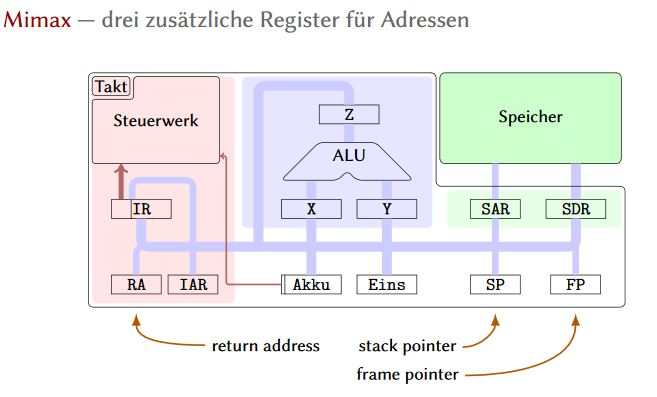
\includegraphics[width=\textwidth]{../topics/mimax/mimax_structure.jpg} 
\end{frame}

\begin{frame}{Neue Befehle}
	\begin{block}{CALL adr}
			\begin{itemize}
				\item ähnlich wie \emph{JMP} adr
				\item zusätzlich wird Inhalt vom IAR ins RA geschrieben
			\end{itemize}
		\end{block}
		
		\begin{block}{RET}
			\begin{itemize}
				\item ähnlich wie \emph{JMP} adr
				\item zusätzlich wird Inhalt vom RA ins IAR geschrieben
			\end{itemize}			
		\end{block}
	\emph{CALL adr} ruft also unsere Subroutine auf und mit \emph{RET} kehren wir von der Subroutine zurück zum Hauptprogramm
	\end{frame}

\begin{frame}{SP und FP}
	\begin{block}{stack pointer}
		zeigt auf Stelle an die \emph{push} den nächsten Wert legen würde\\
		\emph{LDVR disp(SP)} holt oberstes Speicherelement in Akku\\
		\emph{STVR disp(SP)} speichert Akkuinhalt als oberstes Stackelement	
	\end{block}
	\begin{block}{frame pointer}
			funktioniert ähnlich wie SP, genaueres in anderen Vorlesungen
	\end{block}
\end{frame}

\begin{frame}
	Für Beispiele mit der pointer-Magie schaut euch am besten die Vorlesungsfolien an!
\end{frame}

\begin{frame}{Aufgabe}
	\begin{exampleblock}{Aufgabe}
		Schreibe ein Programm, das eine an Adresse $a$ gegebene Zahl mittels einer Subroutine negiert und danach wieder in $a$ speichert. Die Adresse $R$ sei zum Zwischenspeichern frei verfügbar.
	\end{exampleblock}
\end{frame}

\begin{frame}
	\begin{block}{Lösung}
		\emph{main}:LDV $a$\\
		CALL sub\\	
		HALT\\
		\emph{sub}:NOT\\
		STV $R$\\
		LDC 1\\
		ADD $R$\\
		STV $a$\\
		RET
	\end{block}
\end{frame}
